\documentclass[a4paper,twoside]{article}

\usepackage{epstopdf}
\usepackage{epsfig}
\usepackage{subfigure}
\usepackage{calc}
\usepackage{amssymb}
\usepackage{amstext}
\usepackage{amsmath}
\usepackage{amsthm}
\usepackage{multicol}
\usepackage{pslatex}
\usepackage{apalike}
\usepackage{SCITEPRESS}
\usepackage[small]{caption}
\usepackage{epstopdf}

\subfigtopskip=0pt
\subfigcapskip=0pt
\subfigbottomskip=0pt

\begin{document}

\title{Using Agents \& Artifacts to Access the Semantic Web  \subtitle{A Recommender System Case Study} }

\author{\authorname{J\'{e}ssica Pauli de C. Bonson\sup{1}, Elder Rizzon Santos\sup{1} and Ricardo Azambuja Silveira\sup{1}}
\affiliation{\sup{1}Universidade Federal de Santa Catarina (UFSC), Brazil}
\email{\{jpbonson, ersantos, silveira\}@inf.ufsc.br}
}

\keywords{Multi-Agent System, Agents \& Artifacts, Semantic Web, Cartago, Recommender System, Learning Objects}

\abstract{The integration of agents to the Semantic Web can significantly improve the Web services and the Multi-Agent Systems (MAS), by increasing the knowledge available to agents to perform semantic tasks. In this paper we integrate the access of agents to the Semantic Web by means of the Agents \& Artifacts model, using the Cartago framework. To test our approach, our case study is a recommender system to define metadata of a Learning Object according to a metadata standard. Our agents are able to provide recommendations to the user by querying the DBPedia through artifacts. Following the knowledge representation available on the Semantic Web, our artifacts aid the agents on the recommendations by querying linked data sources considering context-specific categories, classes or individuals. The main contribution of our work is to develop a prototype integrating MAS to the Semantic Web using artifacts.}

\onecolumn \maketitle \normalsize \vfill

\section{\uppercase{Introduction}}
\label{sec:introduction}

\noindent In this paper we research the use of the Agents \& Artifacts (A\&A) \cite{ref1} model to ease the access of agents in a Multi-Agent Systems (MAS) to the functionalities of the Semantic Web. To test our approach we adopted the case study of the development of a recommender system for the educational area. The system is able to recommend values for metadata of Learning Objects (LO) based on partial knowledge provided by the user. The agents use the data to query the semantic repository DBPedia through specialized artifacts.

MAS can be defined as a loosely coupled group of autonomous agents that interact in order to solve a problem \cite{ref36}. The A\&A model emerged from the need of modeling the environment of a MAS as a first-class entity \cite{ref7,ref78,ref10,ref3}. Artifacts can model tools and resources to help the agents execute their tasks at runtime. In this work the artifacts model the semantic searches to access the Semantic Web \cite{refOPQ}, more specifically, the DBPedia \cite{refXYZ}. DBPedia is queried to get recommendations for the metadata of a Learning Object (LO). A LO is any resource that may be used in a learning context \cite{ref40}. Metadata provides additional information about a LO, like title, description, keywords, authorship and rights.

The remaining sections of this article are structured as follows: We give an overview of the research background regarding A\&A, Semantic Web and LOs in Section  \ref{sec:background}. Related work is presented in Section 3. Section 4 describes our approach to the access of agents to the Semantic Web and the system implementation. In Section 5 we discuss the results obtained in this work. Section 6 presents our conclusions and outlines future work.


\section{\uppercase{Background}}
\label{sec:background}

\subsection{Agents \& Artifacts}

\noindent In this work we use Jason to develop the MAS agents. Jason \cite{ref35} is an Open Source interpreter for an extended version of AgentSpeak, a logic-based agent-oriented programming language. Given the grounding on AgentsSpeak(L), the agents in Jason follow the BDI model \cite{ref20}. Along with Jason, we adopt the Cartago \cite{refCartago} infrastructure to model the environment as artifacts. Cartago is a platform and infrastructure that provides a general programming model to build working areas where agents can use shared artifacts that represent the environment.

\cite{ref5} discusses two points of views regarding artifacts. From the agents' perspective artifacts are entities that model tools and resources, and are dynamically instantiated, observed, shared, grouped and used in order to help the agents to accomplish their tasks. From the programmer's point of view, artifacts are abstractions to model and implement a working environment that agents can use, so that they can interact with other agents and the external environment.

\subsection{Semantic Web}

\noindent According to the World Wide Web Consortium (W3C), the goal of the Semantic Web is to "allow data to be shared effectively by wider communities, and to be processed automatically by tools as well as manually." \cite{ref53} states that to accomplish this, Semantic Web ontologies are used to provide extensible vocabularies of terms, each with a well-defined meaning. In computer science, an ontology models some aspect of the world by providing a vocabulary that describes the domain being modelled and provides an explicit specification of the intended meaning of that vocabulary \cite{ref53}.

The need for an expressive and standard ontology language leaded to the development of the OWL ontology language standard. OWL uses an RDF-syntax and is based on Description Logics \cite{refDL}. It can represent rich and complex knowledge about things, groups of things, and relationships. Computer programs are able to process the knowledge expressed in OWL to generate logic inferences.

DBPedia \cite{refXYZ} is built upon the Semantic Web, its goal is to extract structured information from Wikipedia and to make this information accessible on the Semantic Web. Currently the DBpedia knowledge base describes over 2.6 million entities, along with their attributes and relationships, in domains such as people, companies, films, and scientific publications. DBPedia employs as its main ontology one that is a mapped version of the Wikipedia templates. Other ontologies are linked to DBPedia, for example, Yago \cite{refYAGO} and FOAF \cite{refFOAF}.

DBPedia provides a public SPARQL endpoint \footnote{http://DBpedia.org/sparql} to query its knowledge base. The triple store OpenLink Virtuoso \cite{refVIRT} is used as the back-end database engine. SPARQL is the standard language for querying RDF data, it is based on graph patterns and subgraph matching \cite{refABC,refDEF}. To query the SPARQL endpoint we adopted Jena API \cite{refJENA}, an open source Java framework for building Semantic Web and Linked Data applications. DBPedia was chosen as our system knowledge base since it is based on Wikipedia, a source frequently used by students to obtain information. Futhermore, DBPedia is considered as one of the most famous basis of the Semantic Web \cite{refEntrevista}.


\subsection{Learning Objects}

\noindent According to the IEEE \cite{ref40} a learning object is "any entity, digital or non-digital, which can be used, re-used or referenced during technology supported learning". Some examples are multimedia content, instructional content, learning objectives, instructional software and software tools. LOs can have additional information about them expressed through metadata.
\cite{ref42} defines metadata as structured data about other data, that can be objective (authors, creation data, version...) or subjective (keywords, abstract...). 

A set of metadata can be grouped into a metadata standard, so that the metadata will have a well-defined semantic in accordance to the view of a specific community. The metadata standards for LOs favor the sharing, cataloguing, discovery and reuse of the learning objects \cite{ref42}. In this work we use the Brazilian standard OBAA \cite{refOBAA}. Our case study is based on the problem of specifying the metadata of a LO according to a metadata standard, so it can be easily shared and understood. This is a very tiresome task \cite{ref38}, which is related to the low production of LOs and frequent creation of LOs that don't follow a metadata standard. 

\section{Related Work}
\label{sec:relatedwork}

\noindent At \cite{refB} the authors developed the agent architecture JASDL (Jason AgentSpeak–DescriptionLogic), an  extension of the Jason agent platform. Their goal is to provide features of agent programming combined with ontological reasoning such as plan trigger generalisation and belief base querying based on ontological knowledge. In order to implement this, the authors used the OWL-API as the DL-Reasoner and improved the Jason belief base with the capacity for ontological reasoning. \cite{refB} considers JASDL as the first full implementation of an agent-oriented programming language with transparent use of ontologies and underlying ontological reasoning within a declarative setting.

At \cite{refC} is proposed Argonaut, a prototype that integrates Jason with the Semantic Web framework Jena to support context aware computing based on OWL ontologies. They developed a MAS for the mobile computing context, where the agents help the users to find out about locally situated services. Argonaut is the first practical approach integrating OWL, Jason and Jena \cite{refC}. In their model, all interactions with ontologies are defined within predefined internal actions in Java.

At \cite{refA} the authors describe ITTALKS, a web-based system that offers accesses to information about talks, seminars and colloquia related to information technology by means of intelligent notifications. To accomplish this, the authors developed a MAS that access the Semantic Web using the DAML (DARPA Agent Markup Language) language. DAML is employed for knowledge base representation, reasoning, and agent communication. By using DAML, the agents at ITTALKS are able to infer extra information about the talks, such as finding talks compatible with the user's interests, schedule, location and current traffic. Other relevant related works can be found in \cite{refD}, \cite{refE} and \cite{refF}

\section{The Recommender Model}

\noindent In this paper we developed a recommender system for the metadata fields of a LO, based on an application profile of the metadata standard OBAA. To generate the recommendations our system uses a MAS composed of agents and artifacts specialized in accessing the DBPedia entities through SPARQL queries. Figure \ref{fig:new1} shows an overview of the system. The user informs the metadata that she already knows to the system and then requests recommendations on other metadata fields, or to improve a metadata field already specified. Next, the GUI gathers the partial knowledge and sends it to the MAS, composed by agents and artifacts. Then the agents use the artifacts to query the DBPedia to find recommendations based on the partial knowledge initially provided. Finally, the recommendations are sent back to the GUI that shows them to the user.

\begin{figure}[!h]
  %\vspace{-0.2cm}
  \centering
   {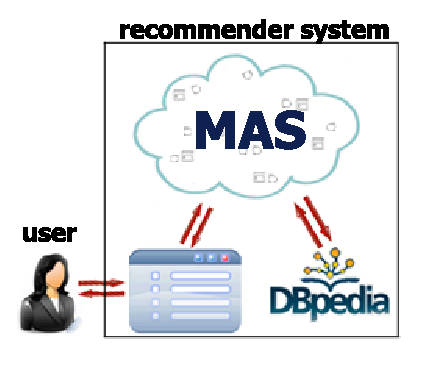
\epsfig{file = figura1icaart.eps, width = 4.0cm}}
  \caption{Overview of the system.}
  \label{fig:new1}
 \end{figure}

We focused on the metadata Title, Description and Keywords of General category of the OBAA profile. We chose them because they are generic and so a wide range of recommendations can be generated for them. In addition, they can be easily mapped to some of DBPedia properties, such as abstract, comment, title, name, and label.

In Figure \ref{fig:new2} is shown the architecture of the recommender model. The cloud represents the MAS, that contains the agents and artifacts. The InputArtifact and the OutputArtifact work as an integration between the MAS and the GUI, they also coordinate the agents. The InputArtifact provides the keywords to them and the OutputArtifact collects the results processed by the agents. The main part of the system is composed by nine agents and artifacts specialized in three types of semantic searches at DBPedia: individuals, classes and categories, where category is an informational structure derived from Wikipedia. Each of these artifacts are mapped to one agent, so the system can process the queries in parallel, because the A\&A model doesn't allow more than an agent using an artifact at a time. The artifacts return the results as the individuals that are more similar to the keyword. It is relevant to notice that all the three artifacts return individuals, in order to group and rank them. So after processing the query the classes and categories obtained by the respective approaches are processed in order to get the individuals that belong to them.

\begin{figure*}[!h]
  %\vspace{-0.2cm}
  \centering
   {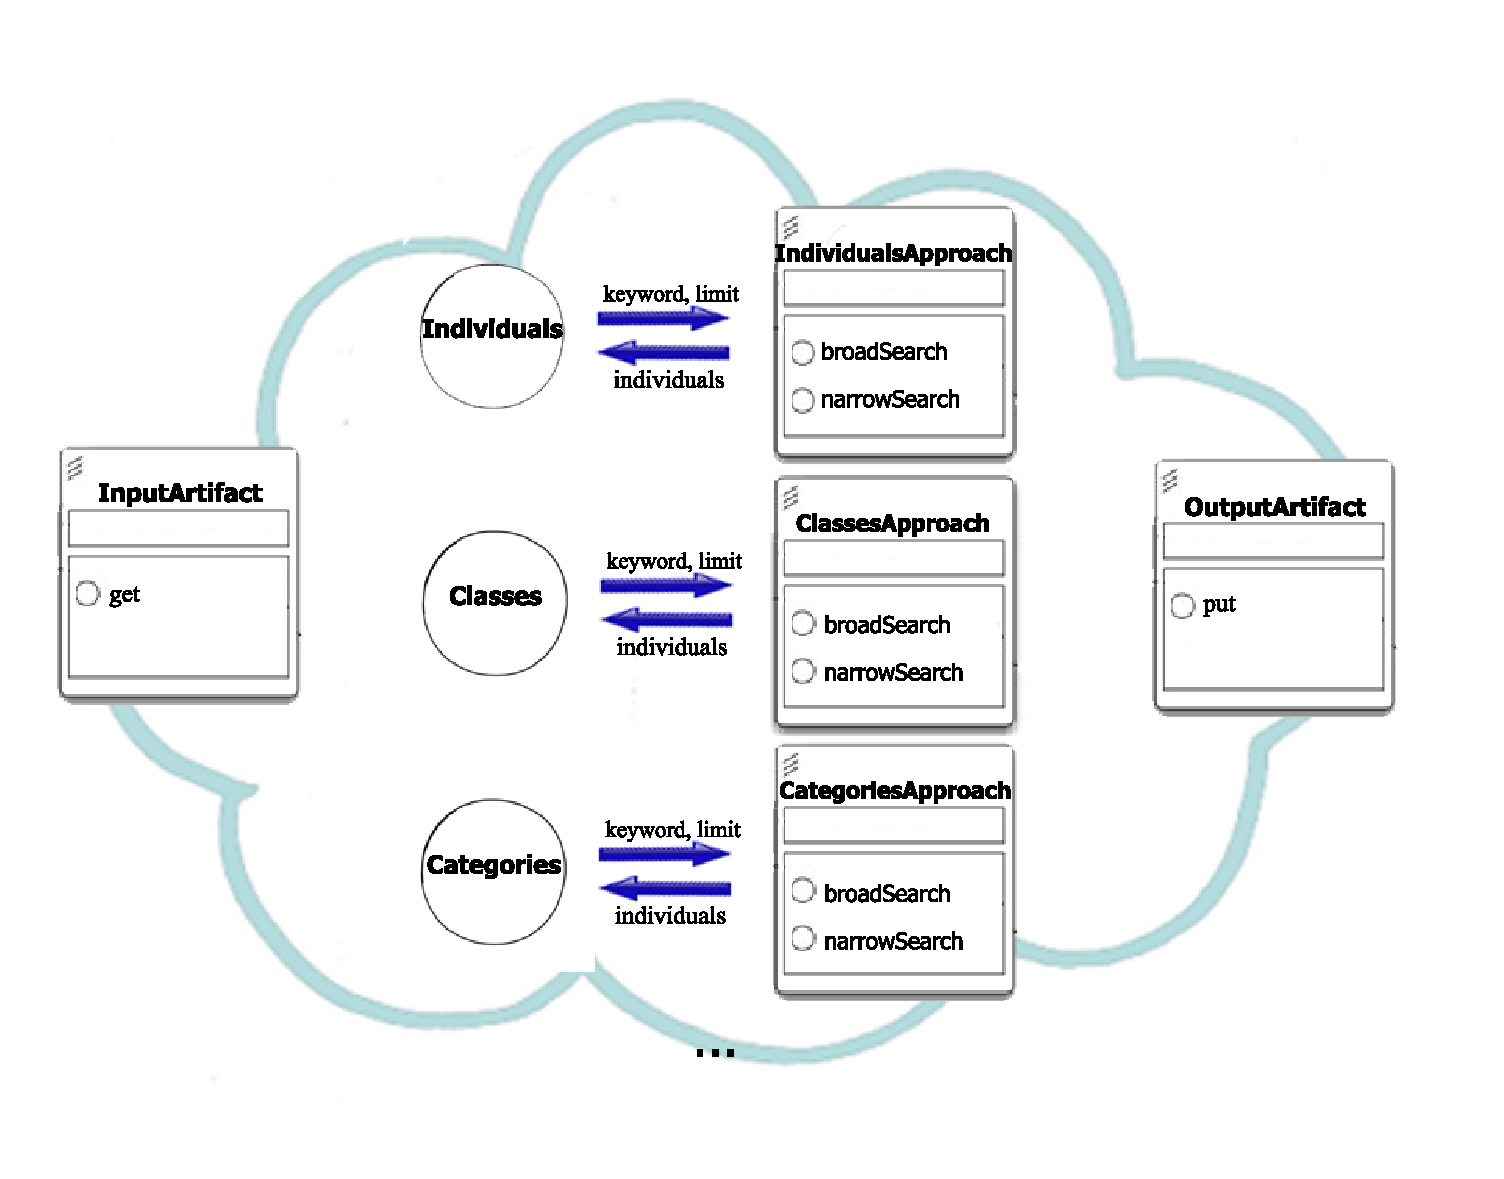
\epsfig{file = figura2icaart.eps, width = 17cm}}
  \caption{Overview of the recommender model.}
  \label{fig:new2}
 \end{figure*}

The workflow of the information exchange works as follows: After partially informing at least one of the three metadata fields, the user can request the system to provide recommendations for one of the three metadata fields. The GUI gathers all the partial knowledge available, along with the fields from where they were obtained, and sends this information to the control layer. The control layer is responsible for processing the partial knowledge of the metadata fields through Natural Language Processing (NLP) in order to obtain keywords. After it, the best eight keywords are sent to the InputArtifact. By best we consider the keywords that showed up more times, so they are more important for the user. We select just a few number of keywords to reduce the processing time.

Every 0.5 seconds the agents check the InputArtifact for available keywords. Each keyword is obtained by three agents, each one specialized in a type of semantic search. The agents process the keywords in parallel through artifacts. After processing the keywords, the artifacts return ontology individuals. They are sent to the OutputArtifact that ranks them and selects the ten best individuals. Those individuals are used to obtain the values from properties that are compatible to the metadata originally requested for recommendations. Finally, the GUI gets the results from the OutputArtifact and shows them to the user.

\subsection{Recommender System}
\label{sec:recsys}

\noindent In our model there are three types of artifacts, each one specialized in a kind of semantic search: by individuals, by classes and by categories. There are three kinds of agents, each one uses a type of artifact. Every artifact provides two ways of performing a semantic search: a broad and a narrow one. The agents access these operations by providing the keyword to be processed and the limit of the search. The broad semantic returns more results, sacrificing quality, and the narrow search get few, higher quality, results.

The main difference between the broad and the narrow semantic search is which and how many filters are employed on the results and the depth used during the search. For example, the broad search for individuals filters the results by the classes they derive from, such as VideoGame, TelevisionShow and Band. To further refine the results, the narrow search filters based on what categories they belong, for example, Sports, Companies and Comics. Our criteria to define the filters are based on if the class or category seemed to be relevant for an educational context.

In the individual approach to semantic search, the keywords are processed in order to obtain individuals that contain the keyword in the properties db-prop:title or db-prop:name. A shorter version of the SPARQL query for the narrow search of this approach is shown below. The words preceded by the symbol @ are parameters that are informed by the agents when calling the artifact's operation. The query starts by stating the prefixes, then it is defined what the query should return at SELECT and which criteria is used during the selection at WHERE. The filters ban the results that belong to prespecified categories. We also use the transitive option on the filters to limit the depth of the search. The parameters that the agent informs to perform the query are @keyword, the keyword being searched; @t\_max, the depth of the search; and @limit, the number of results returned by the query.

\begin{small}
\begin{verbatim}
PREFIX db-prop: <http://dbpedia.org/property/>
PREFIX dbpedia-owl:
   <http://dbpedia.org/ontology/>
PREFIX rdf:
   <http://www.w3.org/1999/02/22-rdf-syntax-ns#>
PREFIX rdfs:
   <http://www.w3.org/2000/01/rdf-schema#>
PREFIX dbpedia_cat:
   <http://dbpedia.org/resource/Category:>
PREFIX dcterms: <http://purl.org/dc/terms/>
PREFIX foaf: <http://xmlns.com/foaf/0.1/>
SELECT distinct ?object
WHERE {
{?object db-prop:title ?title . ?title
   <bif:contains> "+@keyword+" . }
UNION 
{?object  db-prop:name ?name. ?name
   <bif:contains> "+@keyword+" . }
filter (NOT EXISTS
   {?object dcterms:subject ?Category .
   ?Category skos:broader dbpedia_cat:Sports
   option(TRANSITIVE, T_DISTINCT,
   t_max(@t_max)) }) .
filter (NOT EXISTS
   {?object dcterms:subject ?Category .
   ?Category skos:broader dbpedia_cat:Companies
   option(TRANSITIVE, T_DISTINCT,
   t_max(@t_max)) }) .
}
LIMIT @limit
\end{verbatim}
\end{small}

For the classes and categories approaches the goal is to obtain the classes or categories which have the property rdfs:label containing the keyword. Here the difference between the broad and the narrow search is just how many classes or categories are being filtered. The results for the semantic searches are respectively classes or categories, so the agent uses an additional operation on the artifact to obtain the individuals belonging to them.

\subsection{Agents and Artifacts Implementation}
\label{sec:aeaimpl}

\noindent In this section we will describe how we implemented the recommender system according to the A\&A model. The agent initializer instantiates all the artifacts for the MAS: the InputArtifact, the OutputArtifact and nine specialized artifacts, three for each of the three kinds of semantic search. Each type of artifact has three instances in order to improve the parallelism, since just one agent can use an operation in an artifact at a time in the A\&A model. We also create three agents for each type of search, a total of nine specialized agents. In order to the agents to know the names of the artifacts they are going to use, each artifact is instantiated with the same name of the agent that will use it.

Below we show a shorted version of the code for the classes\_approach agent. It starts by discovering the artifacts that it will use through the goal myTools. Those are the artifacts for input, output and one specialized on the classes approach. Then the goal consumeItems checks if new keywords are available in the InputArtifact at 0.5 seconds intervals. When a keyword is obtained it is used in the processItem goal, which executes the semantic search. First, the agent calls the artifact's operation execute\_broad(Keyword, 30, R1), where 30 is the limit of classes that will be returned and R1 is the classes returned by the search. This operation is implemented in Java and uses the Jena API to process the SPARQL query at the DBPedia endpoint. Following the initial operation, the agent uses the results from the broad search to execute a narrow search. If after executing the narrow search there are no results, the agent will send to the OutputArtifact the results from the broad search, otherwise the results from the narrow search will be sent. This decision is made by the goal decideOutcome. Before sending the results to the OutputArtifact through the put operation, the agent calls the operation execute\_getIndividuals(R1, 20, R3) to obtain up to 20 individuals from each class as the final result from the semantic search. The agent code for the individuals and categories approach is similar to the one for the classes approach. The difference for the individual approach is that the final result is already the output from the broad or the narrow searches.

\begin{small}
\begin{verbatim}
!observe.

+!observe : true 
  <- .wait(200); 
    ?myTools(A1, A2, Id);
    !consumeItems(Id).

+!consumeItems(Id): true
<- .wait(500);
get_for_ClassesApproach(Item);
!processItem(Item, Id);
!!consumeItems(Id).

(...)

+!processItem(Keyword, Id) : true
<-  execute_broad(Keyword, 30, R1)
   [artifact_id(Id)];
	execute_narrow(R1, R2)[artifact_id(Id)];
	isEmpty(R2, Test)[artifact_id("input")];
	!decideOutcome(R1, R2, Test, Id).	

+!decideOutcome(R1, R2, Test, Id) : Test
<- execute_getIndividuals(R1, 20, R3)
   [artifact_id(Id)];
	put(R3).

(...)
\end{verbatim}
\end{small}

\subsection{Results Processing}

\noindent The OutputArtifact gathers the resultant individuals from all agents and ranks them to get the ten best ones to generate recommendations. The total score for an individual depends upon what approach generated it:

\begin{equation}\label{eqX}
score = 1.3*(indiv.) + 1*(categ.) + 0.8*(classes)
\end{equation}

The individuals approach receives the higher score since our empirical tests indicate that its results had a better quality, due to the filters being applied directly to the final results. The results from the categories approach were slightly better than the ones from the classes approach, probably because the categories at DBpedia have a stronger basis than the classes, since the categories are derived directly from the Wikipedia and are informative concepts. To define the quality of the results we compared them to a list of items that described general criterias of conceptual similarity to an educational context.

After selecting the ten best individuals the OutputArtifact queries the DBPedia to obtain the values of their properties. The properties queried depend on what metadata field the user requested recommendations for. Just one recommendation is returned per individual, but since there isn't a common property for all individuals the system tries to query different properties until a value is obtained. The queried properties for the Description field are dbpedia-owl:abstract and rdfs:comment. For Title and Keywords the properties used are db-prop:title, db-prop:name, foaf:name and rdfs:label. We query the same properties for both Title and Keywords since we didn't find a property vastly used to represent keywords at DBPedia. Finally, the list of the recommendations and the URI of individuals that generated them is shown to the user in the GUI.

We noticed that the recommendations were useful to obtain more information about a concept or subtypes of a concept, but most of the time they had a bad quality for the educational context. Another problem was that, due to the use of filters to improve the quality of the results, a semantic search could take a long time to process. We believe that these problems happened because DBPedia isn't a semantic repository specific for educational purposes, then lacking the pedagogical information necessary for the recommendations. So, a better quality of recommendations, and a better performance, could be obtained if we query a repository focused on the educational context or specific for LOs.

\section{Results and Discussion}
\noindent In this paper we developed a recommender system where agents access the Semantic Web by means of artifacts that model the environment. The system is able to obtain recommendations for LO metadata using the partial knowledge provided by the user to process semantic queries on DBPedia through SPARQL. The contributions and results of this work can be summarized in three points of view:

a) Metadata recommenders systems: To the best of our knowledge, in the context of recommenders specific for educational LO metadata there are no works available to compare our results with. The system developed in this paper is an initial prototype for this context. In order to offer better recommendations for LO metadata, it would be necessary to evaluate our system accessing a semantic repository specific for the educational context.

b) Recommenders systems in general: In this work our goal was to develop a model that facilitates the access of agents to the Semantic Web, thus obtaining high quality recommendations was not our focus. Therefore we didn't evaluate our system focusing on recommendations, but we could do a proper evaluation in future work.

c) Architectures that enable agents to access the Semantic Web: The main objective of our paper was to developed a model of system where agents can access to the Semantic Web by means of artifacts, so this is the context where we are able to make most of our comparisons. In section \ref{sec:relatedwork} we presented related works where agents access the Semantic Web. The main difference between our work and the previous ones regarding the access to the Semantic Web by agents is that in this work the integration is accomplished by means of artifacts. In this system the artifacts are used as a middleware where the ontological interactions are processed, and additionally as coordinators of the agents.

The semantic artifacts use SPARQL queries with a predefined general structure. In the current version the parts customizable by the agents are the keywords being searched, the prefixes, the filters and some parameters of the search. In a future version we could use the functionality of internal properties of the artifacts. Internal properties can be modified at runtime by agents to change the services being offered by the artifact. So the agents would be able to customize the queries to DBPedia at runtime.

Due to the adoption of artifacts, our model provides reusability: By using the artifacts developed in this model, other agents are able to access the Semantic Web without the need to implement artifacts specific for them. It also isn't necessary to develop a whole new architecture or language in order to agents to access the Semantic Web. Nowadays Cartago, the framework that implements the A\&A model, supports only the Jason agent language, but conceptually any BDI agent is able to use the artifacts developed in this work.

Our main problem with using the A\&A model was that it supports agent using various artifacts at the same time, but an artifact can't be used by more than one agent at a time. To solve this, we instantiated each semantic artifact one time for each agent in our model. The artifacts are instantiated with the name of the agent that will use them, so the agents know what artifact to request. It was an effective approach for our case, but it isn't very elegant and may escalate quickly for a higher number of agents or artifacts.

Other relevant points are that by using artifacts there is less computational burden on the agent side, since they don't need to waste time or resources processing the semantic query. The agents just activate the desired operation at the artifact and they are free to accomplish other goals while the artifact process the query. Finally, there is dynamic extensibility, a feature of the A\&A model that enables agents to create and dispose artifacts by need at runtime. In \cite{ref5} the authors discuss in more details the advantages of the A\&A model.

\section{Conclusion and Future Work}

\noindent In this paper we study the use of the Agents \& Artifacts (A\&A) model to ease the access of agents in a MAS to the functionalities of the Semantic Web, more specifically, of the DBPedia. Our research was tested with the case study of a recommender system for the metadata of Learning Objects (LO) based on the metadata standard OBAA. The agents query the DBPedia through operations available in specialized artifacts. We instantiate three types of artifacts, each one specific for a kind of semantic search: by individuals, classes or categories.

Possible future works for this research include: test the artifacts with other semantic repositories in order to obtain better recommendations; consider more metadata fields in the semantic searches; agents that monitor the GUI and make recommendations at real time; agents configuring the artifacts to modify the structure of the SPARQL queries at runtime; to utilize the contents of the LO or the user's personal data as context; and to make an empirical evaluation of the system.

\vfill
\bibliographystyle{apalike}
{\small
\bibliography{example}}

\vfill
\end{document}

